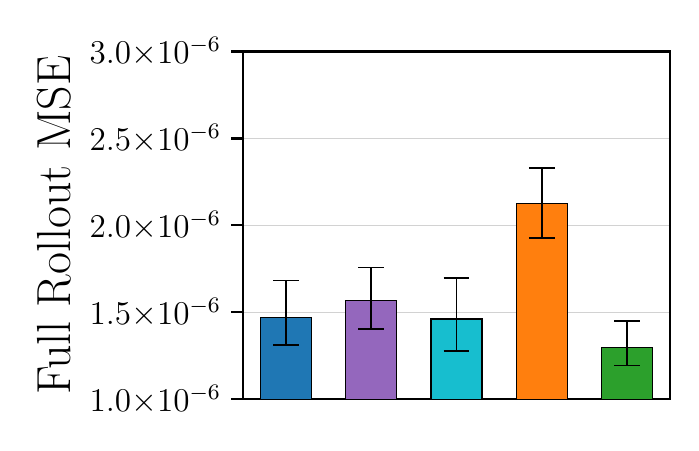
\begin{tikzpicture}
\definecolor{darkgray}{RGB}{169,169,169}
\definecolor{lightgray204}{RGB}{204,204,204}
\definecolor{tabblue}{RGB}{31,119,180}
\definecolor{taborange}{RGB}{255,127,14}
\definecolor{tabpurple}{RGB}{148,103,189}
\definecolor{tabred}{RGB}{214,39,40}
\definecolor{tabcyan}{RGB}{23,190,207}
\definecolor{tabgreen}{RGB}{44,160,44}

\begin{axis}[
    line width=0.8pt,
    axis line style={black},
    height=6cm,
    width=7cm,
    scaled y ticks=false,
    xmin=-0.5, xmax=4.5,
    xtick=\empty,
    ymin=1.0e-6, ymax=3.0e-6,
    ymajorgrids,
    y grid style={lightgray!70},
    tick align=outside,
    ylabel={Full Rollout MSE},
    ylabel style={font=\LARGE, color=black},
    tick label style={font=\large, color=black},
    ytick style={color=black, line width=0.8pt},
    ytick={1.0e-6, 1.5e-6, 2.0e-6, 2.5e-6, 3.0e-6},
    yticklabels={
        \(1.0{\times}10^{-6}\),
        \(1.5{\times}10^{-6}\),
        \(2.0{\times}10^{-6}\),
        \(2.5{\times}10^{-6}\),
        \(3.0{\times}10^{-6}\)
    },
    ytick pos=left,
]

% 0: pointpatch (tab:blue)
\draw[fill=tabblue, draw=black, line width=0.5pt]
    (axis cs:-0.3, 1e-6) rectangle (axis cs:0.3, 1.4707e-6);
% 1: peach_only_ml_and_matprop (tab:purple)
\draw[fill=tabpurple, draw=black, line width=0.5pt]
    (axis cs:0.7, 1e-6) rectangle (axis cs:1.3, 1.5698e-6);
% 2: peach_only_ml_and_sdf (tab:red)
\draw[fill=tabcyan, draw=black, line width=0.5pt]
    (axis cs:1.7, 1e-6) rectangle (axis cs:2.3, 1.4608e-6);
% 3: peach_only_ml (tab:orange)
\draw[fill=taborange, draw=black, line width=0.5pt]
    (axis cs:2.7, 1e-6) rectangle (axis cs:3.3, 2.1269e-6);
% 4: oracle (tab:green)
\draw[fill=tabgreen, draw=black, line width=0.5pt]
    (axis cs:3.7, 1e-6) rectangle (axis cs:4.3, 1.2985e-6);

% Error bars
% 0: pointpatch
\draw[black, semithick] (axis cs:0, 1.3136e-6) -- (axis cs:0, 1.6826e-6);
\draw[black, semithick] (axis cs:-0.15, 1.3136e-6) -- (axis cs:0.15, 1.3136e-6);
\draw[black, semithick] (axis cs:-0.15, 1.6826e-6) -- (axis cs:0.15, 1.6826e-6);
% 1: peach_only_ml_and_matprop
\draw[black, semithick] (axis cs:1, 1.4025e-6) -- (axis cs:1, 1.7580e-6);
\draw[black, semithick] (axis cs:0.85, 1.4025e-6) -- (axis cs:1.15, 1.4025e-6);
\draw[black, semithick] (axis cs:0.85, 1.7580e-6) -- (axis cs:1.15, 1.7580e-6);
% 2: peach_only_ml_and_sdf
\draw[black, semithick] (axis cs:2, 1.2787e-6) -- (axis cs:2, 1.6967e-6);
\draw[black, semithick] (axis cs:1.85, 1.2787e-6) -- (axis cs:2.15, 1.2787e-6);
\draw[black, semithick] (axis cs:1.85, 1.6967e-6) -- (axis cs:2.15, 1.6967e-6);
% 3: peach_only_ml
\draw[black, semithick] (axis cs:3, 1.9261e-6) -- (axis cs:3, 2.3300e-6);
\draw[black, semithick] (axis cs:2.85, 1.9261e-6) -- (axis cs:3.15, 1.9261e-6);
\draw[black, semithick] (axis cs:2.85, 2.3300e-6) -- (axis cs:3.15, 2.3300e-6);
% 4: oracle
\draw[black, semithick] (axis cs:4, 1.1949e-6) -- (axis cs:4, 1.4497e-6);
\draw[black, semithick] (axis cs:3.85, 1.1949e-6) -- (axis cs:4.15, 1.1949e-6);
\draw[black, semithick] (axis cs:3.85, 1.4497e-6) -- (axis cs:4.15, 1.4497e-6);

\end{axis}
\end{tikzpicture}